% 
% Annual Cognitive Science Conference
% Sample LaTeX Paper -- Proceedings Format
% 

% Original : Ashwin Ram (ashwin@cc.gatech.edu)       04/01/1994
% Modified : Johanna Moore (jmoore@cs.pitt.edu)      03/17/1995
% Modified : David Noelle (noelle@ucsd.edu)          03/15/1996
% Modified : Pat Langley (langley@cs.stanford.edu)   01/26/1997
% Latex2e corrections by Ramin Charles Nakisa        01/28/1997 
% Modified : Tina Eliassi-Rad (eliassi@cs.wisc.edu)  01/31/1998
% Modified : Trisha Yannuzzi (trisha@ircs.upenn.edu) 12/28/1999 (in process)
% Modified : Mary Ellen Foster (M.E.Foster@ed.ac.uk) 12/11/2000
% Modified : Ken Forbus                              01/23/2004
% Modified : Eli M. Silk (esilk@pitt.edu)            05/24/2005
% Modified: Niels Taatgen (taatgen@cmu.edu)  10/24/2006

%% Change ``a4paper'' in the following line to ``letterpaper'' if you are
%% producing a letter-format document.








%% --------- Short APA CITE Helpfile  --------- %%
%% 	Command									Result
%%	\cite<e.g.,>[p.~11]{Jone01,Ross87}				(e.g., Jones, 2001; Ross, 1987, p. 11)
%%	\citeA<e.g.,>[p.~11]{Jone01,Ross87}				e.g., Jones (2001); Ross (1987, p. 11)
%%	\citeauthor<e.g.,>[p.~11]{Jone01,Ross87}			e.g., Jones; Ross, p. 11
%%	\citeyear<e.g.,>[p.~11]{Jone01,Ross87}			(e.g., 2001; 1987, p. 11)
%%	\citeyearNP<e.g.,>[p.~11]{Jone01,Ross87}		e.g., 2001; 1987, p. 11
%%	\citeNP<e.g.,>[p.~11]{Jone01,Ross87}			e.g., Jones, 2001; Ross, 1987, p. 11
%%


\documentclass[10pt,letterpaper]{article}

\usepackage{cogsci}
\usepackage{pslatex}
\usepackage{apacite}
\usepackage{graphicx}
\usepackage{color}
\usepackage{amsmath}
\usepackage{multirow}
\usepackage{amssymb}
%\usepackage{url}
%\usepackage{hyperref}


 
\definecolor{Red}{RGB}{255,0,0}
\newcommand{\red}[1]{\textcolor{Red}{#1}}  
\definecolor{Green}{RGB}{10,200,100}
\newcommand{\ndg}[1]{\textcolor{Green}{[ndg: #1]}}


%\title{ Lay theories of emotion in explaining behavior }
\title{ Where is the Love (in folk psychology)? \\ Emotions in lay explanations of behavior \ndg{the cute part is a stretch... how about just the second part?}}
 
\author{{\large \bf Desmond C. Ong (dco@stanford.edu)} \\
{\large \bf Jamil Zaki (jzaki@stanford.edu))} \\
{\large \bf Noah Goodman (ngoodman@stanford.edu)} \\
  Department of Psychology, Stanford University, Stanford CA, USA 
}

\begin{document}

\maketitle

\begin{abstract}
Humans use rich intuitive theories to explain the behavior of those around them. Previous work in lay psychology of behavior have tended to treat emotion as an uninteresting cause of unintentional behavior (e.g., being sad causes one to cry), neglecting how people incorporate emotions into explanations of rational, intentional actions. Here, we provide preliminary explorations into integrating emotions into an intuitive belief-desire psychology. Specifically, we show that in the lay theory, people are willing to endorse emotions as causes of intentional actions. Moreover, people readily attribute beliefs and desires as explanations for emotional expressions. This work provides a first step in elaborating people's rich understanding of emotions as an important component of intuitive social cognition.

\textbf{Keywords:} 
Intuitive Psychology, Emotions, Affective Cognition, Explanations
\end{abstract}

% Outline of paper

% More free-form
% Expt 1a) Emotions --> Actions
% Expt 1b) Generate cause of Actions. Coded into emotions, beliefs, situational factors, etc.

% More hypothesis driven
% Expt 2) From Actions / Expressions / Behavior, rate abstract causes: Beliefs, Desires, Emotions, Situation factors

% old
% Expt 2a) Actions / Expressions / Behavior, generate causes: Beliefs, Desire, Emotion, Situation factor
% Expt 2b) From 2a, for all actions/expressions/behavior, pick top b,d,e,s. Find endorsement rates of posterior using sliders.




\begin{quote}
\textit{``... men in rage strike those that wish them best"} 
--- Iago, in Shakespeare's \textit{Othello}, perhaps subtly presaging the (Iago-instigated) murder of Desdemona by Othello's hands. (Shakespeare, trans. \citeyearNP{Othello}, 2.3.205) %(Act 2, Scene 3, line 205) \red{to fix: proper citation}
\end{quote}


%2.3.205 % act 2, scene 3, line 205

%\ndg{this intro is good, though i think it could be made more crisp, and perhaps shortened. clearly identifying the core questions that need to be answered to incorporate emotion in intuitive psychology would help: are there actions causally influenced by emotions but not beliefs and desires? are intentional actions actually independent of emotions? i think laying out the three models in the next section here would make this easier. }

We have a rich intuitive understanding of others and their emotions \cite{Ong2015AffCog}. In his plays, the Bard of Avon makes masterful use of the layperson's understanding of emotion: in \textit{Othello}, the audience is privy to Iago's deliberate manipulation of Othello's jealousy and rage, and can effortlessly predict Othello's murder of Desdemona before it happens. Consider the counterfactual scenario: would Othello still have killed Desdemona had he not been feeling those emotions? This seems unlikely; intuitively, emotions played a key, irreplaceable role in Othello's decision making process.

We naturally extend this type of powerful reasoning to explain the behavior of others, both fictional and nonfictional. This process of reasoning about the mental states and behavior of others is often called folk, intuitive, or lay psychology \cite<e.g., >{Heider1958, Malle2011}. Many modern theories posit a ``belief-desire psychology" \cite<e.g., >{Bartsch1995, Dennett1989, Gopnik1997, Malle1999, Malle2011, Searle2001}, in which an agent has a set of goals (often termed \textbf{desires}), and a set of ideas or beliefs about the world on how to achieve those goals (often termed \textbf{beliefs}). The agent then forms an intention to act upon his beliefs to achieve his desires, resulting in \textbf{intentional action}.
%The tendency of laypeople to attribute such \textit{intentionality} to others forms what \citeA{Dennett1989} famously termed an ``intentional stance", is pervasive and arises as early as 12 months of age \cite{Gergely1995}. 
When laypeople are asked to explain an agent's behavior, they often appeal to both the beliefs and desires of the agent: ``Sue went to the store at 3pm, because (1) she wanted a drink, and (2) she thinks that the store sells alcohol".
%Laypeople also offer as explanations upstream events that resulted in beliefs or desires (\citeNP{Malle1999}'s \textit{Causal History of Reasons}): ``Sue had a bad argument (which caused her to want a drink)", or ``Sue goes to the store everyday (so she knows it sells alcohol)". A fourth class of explanations that laypeople give are \textbf{Enabling Factors}: events that facilitated the feasibility of the intentional action, but did not instigate it: ``Sue got out of work early (which allowed her to go get a drink at 3pm)". 
%Finally, 
\textbf{Unintentional behavior}, on the other hand, are often described as a result of \textbf{situational factors} via physical causality (or \textit{impersonal causality}; \citeNP{Heider1958}): ``Sue slipped and fell because there was ice on the floor (not because she intended to)". This taxonomy\footnote{There are also other explanations that people give for intentional actions, such as upstream events that result in beliefs or desires (\citeNP{Malle1999}'s ``Causal History of Reasons") and events that facilitated but not instigated the action (often called Enabling Factors) that we do not discuss in this paper.} has proven incredibly fruitful and productive in explaining how lay people explain behavior.


%Let us begin by writing down several models which provide more concrete hypotheses. The first model, built off the literature on belief-desire psychology, posits that lay people distinguish two distinct processes that result in two types of behavioral responses (see Fig. \ref{ModelsOfBehaviorFig}a). The first of these two processes assumes that agents have \textbf{Beliefs} and \textbf{Desires}, which interact, giving rise to \textbf{Intentional Actions}. The second process, by contrast, relies on mere causality, and results in a second type of behavioral response. Here, we specifically distinguish between two types of ``other causes", \textbf{Emotions} (e.g., sadness) and \textbf{Situational Factors} (e.g., the ground is icy), and two types of behavior: \textbf{Emotional Expressions} (e.g., crying, laughing), and \textbf{Unintentional Behavior} (e.g., slipping on ice, snoring). Previous theories have subsumed Emotional Expressions into Unintentional Behavior: here, we assume that the former is only caused by emotions, whereas the latter could be caused by situational factors and possibly, emotions (this is to allow emotions to explain unintended ``irrational" behavior). Notably, in these theories of folk psychology, there is no place for emotions in the ``rational" decision making process that humans reason with when explaining the actions of others.

Sadly, these models are often emotionless\footnote{pun intended} and relegate emotions to the bin of other, situational causes. In these models, feeling sad makes one cry, an automatic and ``unintentional" behavior that is out of the control of the agent. There is an implicit assumption that emotion-driven behavior is unintentional, or otherwise ``irrational". See Figure \ref{ModelsOfBehaviorFig}a for an illustration. Here, we specifically distinguish \textbf{Emotions} (e.g., sadness) from \textbf{Situational Factors} (e.g., the ground is icy). Additionally, although most theories do not differentiate \textbf{Emotional Expressions} (e.g., crying, laughing) from \textbf{Unintentional Behavior} (e.g., slipping on ice, snoring), we specifically separate them in this model. Importantly, this model is an insufficient description as it does not account for how lay people use emotions in causal explanations, such as how an agent's emotional state might influence the formation of intentions. Returning to the example of Othello, we argue that even his beliefs (that Desdemona cheated on him) and his desires (perhaps, to punish her) alone, without any rage, would not have led him to murder his wife. 

%Laypeople do have this intuition that emotions influence intentional actions (``he replied my email; the boss must be in a good mood today"). 



%and this has made its way into legal attributions of guilt and responsibility, as in crimes of passion like Othello's. \textit{\red{I need to work on this last line, and crime might not be the best way to end here...}}


How can we incorporate emotions into an intuitive psychology of behavior? In this paper, we seek to explore two hypotheses. First, are intentional actions actually independent of emotions? It is worth noting that many scientific theories of emotion include both ``automatic" and ``intentional" behavior as a crucial part of their definitions of emotion. On one hand, emotions cause characteristic ``automatic" behavioral responses like facial expressions and vocalizations \cite<e.g.,  >{Ekman1992}. On the other hand, emotions also bias agents towards certain types of actions via \textit{action tendencies} \cite{Frijda1989, Fontaine2007} or approach/avoid motivations \cite<e.g., >{Carver2004}. For example, being in a state of happiness predisposes one towards helping others \cite{Isen1972} and risk-taking \cite{Isen1983}. Emotions have already been incorporated into psychological \cite<e.g., >{Schwarz2000emotion}, economic \cite<e.g., >{Loewenstein2003affect}, and philosophical \cite<e.g., >{Zhu2002emotion} theories of behavior, but not yet into an intuitive theory of behavior. Consider Figure \ref{ModelsOfBehaviorFig}b, which posits an intuitive theory in which emotions directly influence the intentional decision making process---in the Discussion, we return to how exactly this influence might occur. %Here, we simply assume that emotions somehow influences the intentional decision making process
\ndg{if emotion (only) directly influences desire, would we count it as model b? if so we need another arrow. anyhow we should make this case clear, since it's plausible...}


% that emotions do play an important role in the formation and execution of intentional action. 


%

%these expressions are also influenced by cultural display rules \cite<e.g., >{Matsumoto1990} and other top-down cognitive processes.

%but it is unclear how a theory of folk psychology incorporates emotions into the lay model of decision making \cite{Ong2015AffCog}. 

Second, are emotion-caused actions---specifically, emotional expressions---independent of beliefs and desires in the intuitive theory? Indeed, emotional display rules \cite<e.g., >{Matsumoto1990} and deliberate deceptive strategies \cite<e.g., >{Depaulo2003} are but two of the top-down cognitive processes that influence ``automatic" emotional expressions. Figure \ref{ModelsOfBehaviorFig}c illustrates this possibility by allowing an agent's beliefs and desires to influence their emotional expressions.
%A third possibility that we must also consider is that the distinction between intentional action and emotional expressions in the lay theory is needlessly strong (Fig. \ref{ModelsOfBehaviorFig}c), and that emotions, as well as beliefs and desires, impact both an agent's intentional actions and emotional expressions. 
% do impact an agent's displayed emotional expressions, and might very well be an important factor in lay explanations of behavior. %However, we (as have many theorists before us) reject the notion that all instances of emotional expressions are intentional, and hence should not be a subset of intentional action.
\ndg{what do you think about adjusting the diagram for model c to have one big node for "Intentional and Emotional Action"? this simplifies the diagram and makes the claim clearer (that there are not actually two kind of actions there).} \red{[DO: I'm a bit uncomfortable with that, as not all emotional expressions are intentional. JZ, thoughts?]}



%moral evaluations (Knobe, 2003)


%\section{Three possible theories of behavior}


\begin{figure}[htb!]
\begin{center}
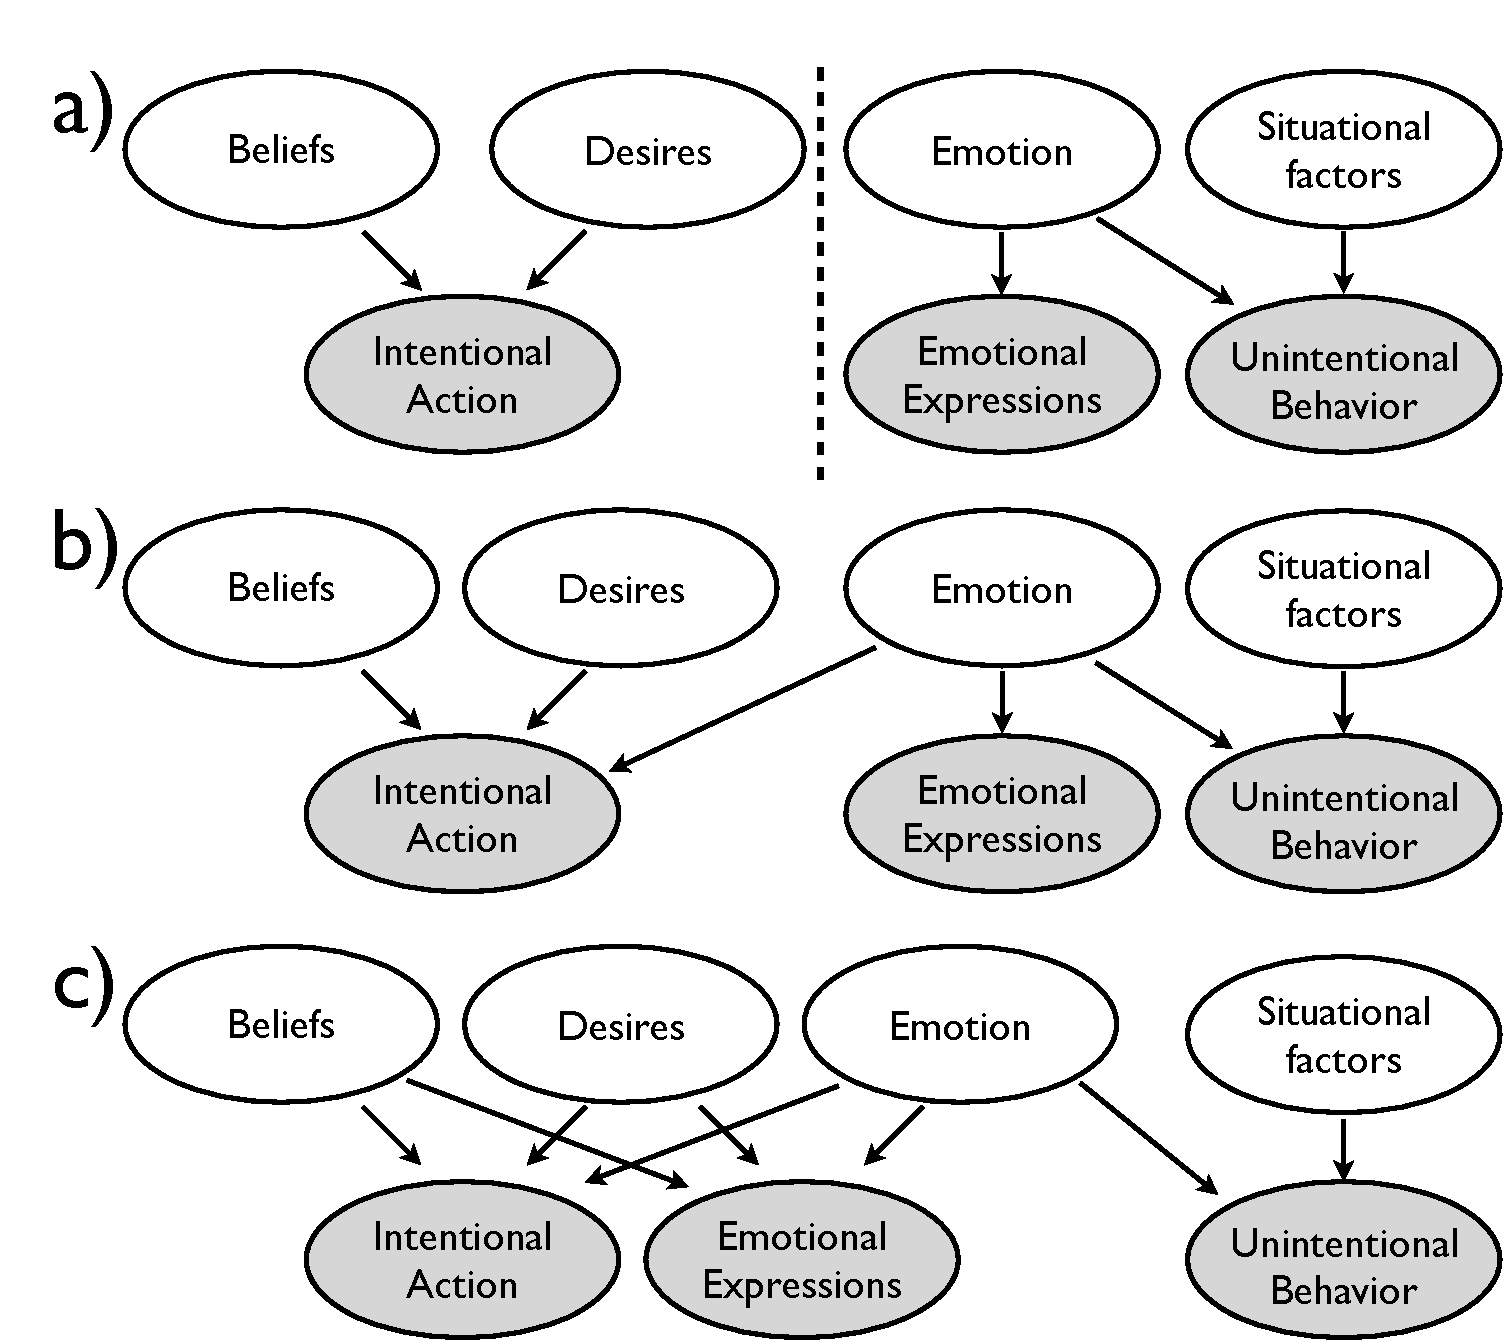
\includegraphics[width=1\columnwidth]{images/model1.pdf} 
\end{center}
\caption{ Possible lay theories of behavior. (a) There are two distinct types of behavioral responses; on the left, the intentional decision-making process that results in intentional action from beliefs and desires. On the right, unintentional behavior and emotional expressions are simply caused by situational factors and emotions via simple causality, without the need for an agent's intentionality. (b) Emotions influence the intentional decision making process. (c) Beliefs and desires also cause emotional expressions. }
\label{ModelsOfBehaviorFig}
\end{figure}


%\ndg{i think this section should probably be re-integrated with the intro, since it will help clarify the options in the intro (and thus make the intro shorter!)...}




In this paper we provide some preliminary explorations of how emotions are incorporated into the intuitive belief-desire psychology, and specifically, how emotions are used or judged as explanations of intentional actions. First, we begin by laying out three possible models: each provides distinct, testable predictions that we explore via experiments with lay participants. In Study 1, we study the types of actions that laypeople think emotions cause, and show that the top emotion-caused actions are judged to have been caused by emotions only about half the time. In Study 2, we show that laypeople are willing to endorse emotions as causes of intentional actions. We also find that people are willing to endorse beliefs and desires as likely causes of emotional expressions (e.g., smiling), which has previously been treated as unintentional behavior in previous lay theories. This paper provides but a first step in exploring how emotions are used by laypeople in explaining behavior, and we end by discussing future directions that are inspired by this research.


%In order to test this, we used a free-response paradigm to have lay people generate actions from emotions (Study 1a), and causes of these actions (Study 1b), to show that emotion-caused actions are judged likely to be caused by other, non-emotional causes. We then tested the three models more rigorously by elicited judgments of explanations of intentional actions, emotional expressions, and unintentional behavior (Study 2).


%%%%

\section{Study 1a: Emotions to Actions}

	In Study 1a, we elicited the actions that participants thought would be caused by different emotions. We then obtained judgments of the counterfactual likelihood (i.e., how likely were these actions if the agent had not felt the emotion). This allowed us to both find the emotions most likely to be ``emotion expressions'' (as described above) and explore whether the emotion is causally necessary to bring about these actions (via the counterfactual judgments).\footnote{Samples of all studies reported in this paper are available at: https://github.com/desmond-ong/shakespeare/}

% Expt 1a) Emotions --> Actions
% Expt 1b) Generate cause of Actions. Coded into emotions, beliefs, situational factors, etc.

\subsubsection{Participants and Procedures.} 
We recruited 100 participants (99\% had English as their native language) through Amazon's Mechanical Turk (AMT). Participants saw statements of the form ``Bob \underline{\hspace{3em}} because he was [\textbf{emotion}]", and were asked to give sentence completions. The presented \textbf{emotion} was one of: \{happy, calm, angry, sad, surprised\}\footnote{We chose a high-arousal positive valence (``happy"), a low-arousal positive valence (``calm"), a high-arousal negative valence (``angry"), a low-arousal negative valence (``sad"), and a high-arousal neutral valence (``surprised") emotion.}. On each page, participants saw only one emotion, and gave 5 different completions (for a total of 25 completions). The emotions were presented in a random order; names were randomized on every sentence.

After participants had given completions to all 5 emotions, they were then presented their answers, and asked to rate the likelihood of the counterfactual: ``You wrote that `\textit{Bob [cried] because he was [sad]}'. If Bob was not feeling [sad], would he still have [cried]?" Participants gave responses on a 7 point Likert scale from ``Very Unlikely" to ``Very Likely". 




\subsubsection{Results.} 
We grouped similar free-responses together (e.g., ``smiled", ``smiled widely", and ``beamed"), and present the top 5 responses for each emotion in Table \ref{Study1aResultsTable}. 
\ndg{need to say more clearly the criteria for grouping and who did it.... ideally we will get this done by naive coders (eg on turk), or automated (eg via synsets).}
Note that, as expected, the majority of these modal responses would easily be judged to be \textit{emotional expressions}: some notable exceptions are ``killed himself"\footnote{It is unfortunate that this is one of the modal lay responses for what an agent will do when he is sad...}, ``punched the wall", ``slept", and ``sat down".


\begin{table}
\scalebox{0.80}{
\begin{tabular}{l l l l l}
\textbf{Happy} & \textbf{Calm} & \textbf{Sad} & \textbf{Anger} & \textbf{Surprised} \\
smiled: 63 & relaxed: 50 & cried: 97 & ``hit X": 56 & jumped: 65 \\
laughed: 51 & slept: 46 & frowned: 17 & yelled: 54 & laughed: 41 \\
\multirow{2}{*}{jumped: 42} & \multirow{2}{*}{sat down: 32} & killed & \multirow{2}{*}{screamed: 21} & \multirow{2}{*}{screamed: 30} \\
& & himself: 13 & & \\
danced: 22 & smiled: 26 & slept: 13 & cried: 15 & yelled: 25 \\
cried: 21 & sighed: 10 & yelled: 13 & cursed: 12 & smiled: 23 \\
\end{tabular}
}
\caption{ Action nominations from emotions (Study 1a). Top 5 responses for each emotion, with nomination counts in parentheses. The most common responses for anger were variants of ``hit X", where X is an object or person (of these, the modal response was: ``punched the wall"). }
\label{Study1aResultsTable}
\end{table}

%\multirow{2}{*}{text}

%%NOTE: this is false:
%The free response portion allowed us to test sufficiency: if a participant nominated an action $a$ when given emotion $e$, then the emotion $e$ is sufficient to have caused that action $a$. 

We turn next to the counterfactual rating task, to investigate necessity of emotion for the elicited actions. 
\ndg{it's probably worth first saying something about the absolute ratings for the modal actions -- this is what we really care about, though lacking any calibration it's hard to draw conclusions...}
We hypothesized that the more often a particular action $a$ is nominated for emotion $e$ across all participants, the more \textit{necessary} is emotion $e$ for action $a$ to occur. Hence, we should expect that these commonly nominated actions $a$ would be less likely to happen in the absence of emotion $e$. In order to test this, we regressed participants' counterfactual likelihood ratings (i.e., how likely is the action to occur if the emotion was absent, $P(A | \neg E)$) against the frequency of that action being nominated across the sample, with random intercepts by participant and emotion. We find that, across all emotions, the more frequently an action is nominated, the less likely participants rate it to occur in the absence of the emotion $(b = -0.0084, 95\% \text{ CI}: [-0.0108, -0.0060], t=-6.82, p<0.001$; See Fig. \ref{Study1aResultsFig}). Thus, the modal nominated actions are judged less likely to occur in the absence of the corresponding emotions, and thus, in participants' lay theories, the corresponding emotions are more necessary for these actions to occur: we shall use this result in Study 1b.



\begin{figure}[htb!]
\begin{center}
	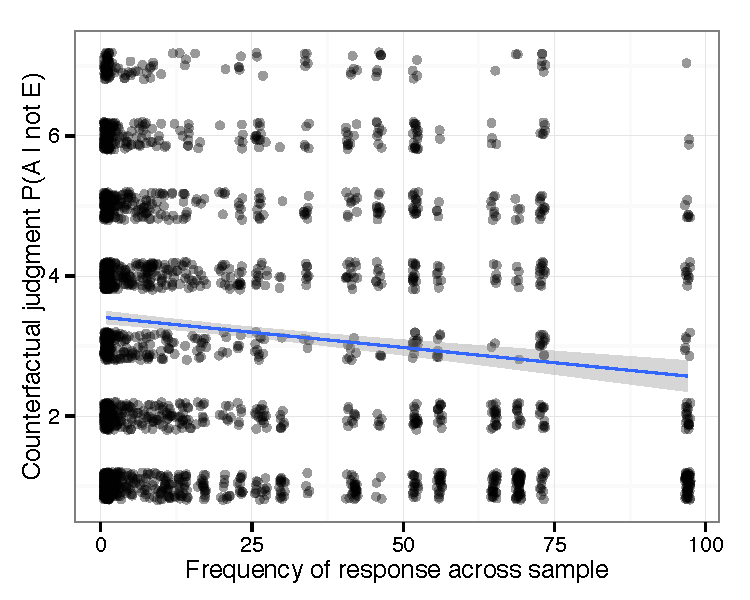
\includegraphics[width=1\columnwidth]{images/study1a_results.pdf}
\end{center}
\caption{ Study 1a Results. Individual counterfactual likelihood ratings ($P(A | \neg E)$) against frequency of an action's nomination across the sample. Data points are transparent and jittered for clarity. }
\label{Study1aResultsFig}
\end{figure}


\section{Study 1b: Causes of Actions}

In Study 1b, we recruited a separate group of participants to give explanations for the modal actions nominated from Study 1a. 
This allows us to explore sufficiency of emotions to cause the actions elicited above, and to test among causal models of ``emotional expressions.''
If Model 1 (Fig. \ref{ModelsOfBehaviorFig}a) is correct then in Study 1b we should only find explanations due to emotions (and perhaps, situational factors), and not explanations that appeal to beliefs or desires.
%	Lay participants from Study 1a judged emotions to be necessary for these modal actions to occur: hence, 


\subsubsection{Participants and Procedures.} 
We recruited 100 participants through AMT (98\% had English as their native language). This time, participants saw statements of the form ``Bob [\textbf{action}] because \underline{\hspace{3em}}", and were asked to complete the sentence. The presented \textbf{action} was one of the fifteen actions drawn from the most popular responses from Study 1a (i.e., the 15 unique actions in Table \ref{Study1aResultsTable}, with ``punched the wall" used in place of ``hit X"). Participants gave 1 completion per action and saw the actions in a random order.

\subsubsection{Results.} 
The free-response completions were coded into one of five categories: (a) ``\textbf{Emotion}" (if there was a mention of an emotion word), (b) ``\textbf{Cause of Emotion}" (if there was a mention of an event that would cause an emotion, e.g., ``his dog died"), (c) ``\textbf{Physical state}" (if the explanation referenced a physical state like tiredness or pain), (d) ``\textbf{Mental state}" (if the explanation referenced a desire or a belief); (e) ``\textbf{Situation}" (for enabling and other situational factors). 
\ndg{same comment about coding. even more so, since there is some judgement involved in eg deciding whether a situation factor is a cause of emotion or just a situation....}

The distribution of coded free-responses is given in Figure \ref{Study1bResultsFig}. \ndg{i like this figure!}
If the actions generated from Study 1a were characteristic of those emotions, and if they could only have been caused by emotions (i.e., Fig. \ref{ModelsOfBehaviorFig}a), then we should expect the vast majority of the explanations to be due to emotions, or to upstream causes of emotions\footnote{``Because he is sad" is a somewhat unsatisfying explanation to ``why is he crying?" in conversation, and often begs the question ``well, so what made him sad?". People often give Causes of Emotion as explanations for (obvious) emotions, and so we decided to code specifically for these.}. However, we see that in fact, only 40.7\% of explanations appeal to an Emotion, and 51.7\% appeal to either an Emotion or to a Cause of an Emotion. There are many references to Physical states (e.g. physical pain as a cause for ``cursing" or ``yelling"; fatigue as a cause of ``sat down" or ``slept"), or to Mental states (e.g. a belief or a desire). Thus, it seems very likely that lay people's judgments of emotion-caused actions are not, in fact, predominantly caused only by emotions. 
The results of Studies 1a-b provides some preliminary support for the model in Figure \ref{ModelsOfBehaviorFig}c, which does not distinguish intention-caused from emotion-caused actions. 
We test this model more precisely in Study 2.

\begin{figure}[htb!]
\begin{center}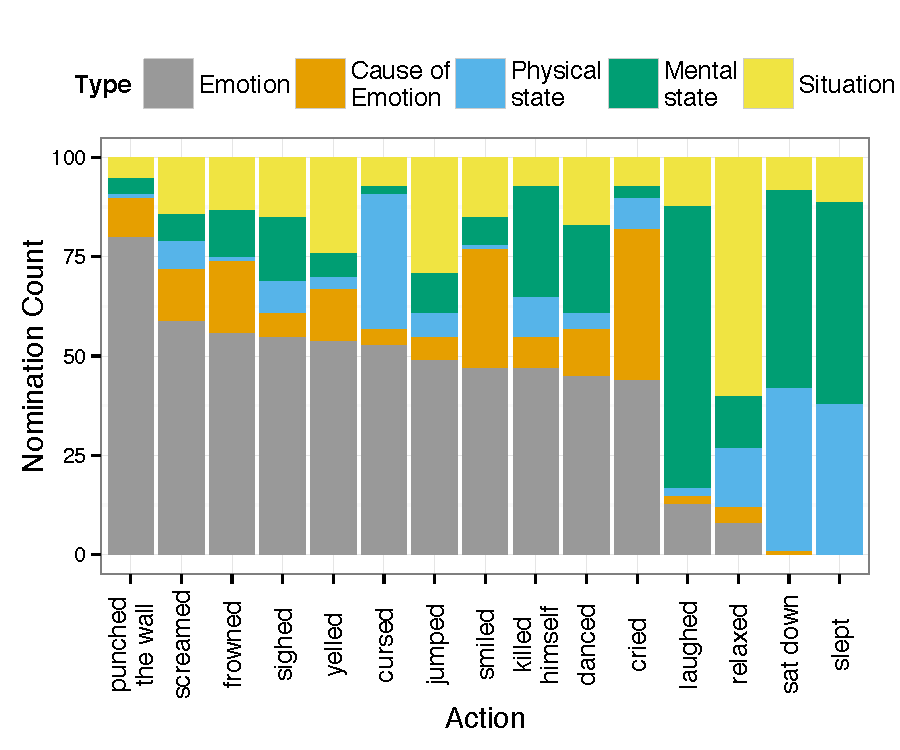
\includegraphics[width=1\columnwidth]{images/study1b_codePlot.pdf}\end{center}
\caption{ Results of Study 1b. We plot the number of explanations that fall into each type for each action. }
\label{Study1bResultsFig}
\end{figure}


\section{Study 2: Rating explanations for actions}


%In Study 1a/b, we examined participants' judgments of actions from several emotions, and we did not impose any formal structure on the type of actions that people generated (e.g., whether they were intentional actions or emotional expressions). 
In Study 2, we explored a broader set of actions, in order to further test the models in Figure \ref{ModelsOfBehaviorFig}. We chose a set of actions comprising Intentional Actions, Emotional Expressions, and Unintentional Behavior, and asked participants to rate how likely it was that each action was caused by Belief, Desire, Emotion, and Situational Factor explanations\footnote{Although the three models do not differentiate between the causes of Unintentional Behavior, we included Unintentional Behavior and Situational Factors in order to calibrate against baseline predictions that all three models should make.
}. First, we aimed to determine if people judge emotions as suitable explanations for intentional behavior. Second, we aimed to confirm the finding from Study 1 that people will judge beliefs and desires as suitable explanations for emotional expressions. 
Specifically, we would predict, under the model in Figure \ref{ModelsOfBehaviorFig}c, that:
%\ndg{predictions should be introduced in intro to the expt. and probably can be in less detail than here...}
%Importantly, if the model in  was correct, we might hypothesize that: 
\begin{enumerate}
\item For Intentional Actions, %(1st row), 
\textbf{B}eliefs and \textbf{D}esires will be rated as the most likely causes, and \textbf{E}motion ratings will be in the middle. %($B,D>E>S$)
\item For Emotional Expressions, %(2nd row), 
\textbf{E}motion explanations will be rated as the most likely, while ratings of \textbf{B}eliefs and \textbf{D}esires will be endorsed to a small extent. %($E \gg B,D>S$)
\item For Unintentional Behavior, %(3rd row), 
we should see high ratings for \textbf{S}ituational Factor causes, and low endorsements for other types of causes. %($S\gg B,D,E \sim 0$)
%\item Ambiguous Behavior (4th row) were judged by previous participants \cite{Malle1999} as being intentional and others as being unintentional. Thus, we hypothesized to see a mix of responses for Intentional and Unintentional. Averaging across many participants, this should result in mediocre ratings for all four types of causes. ($B=D=E=S > 0$)
\end{enumerate}


\begin{figure*}[htb!]
\begin{center}
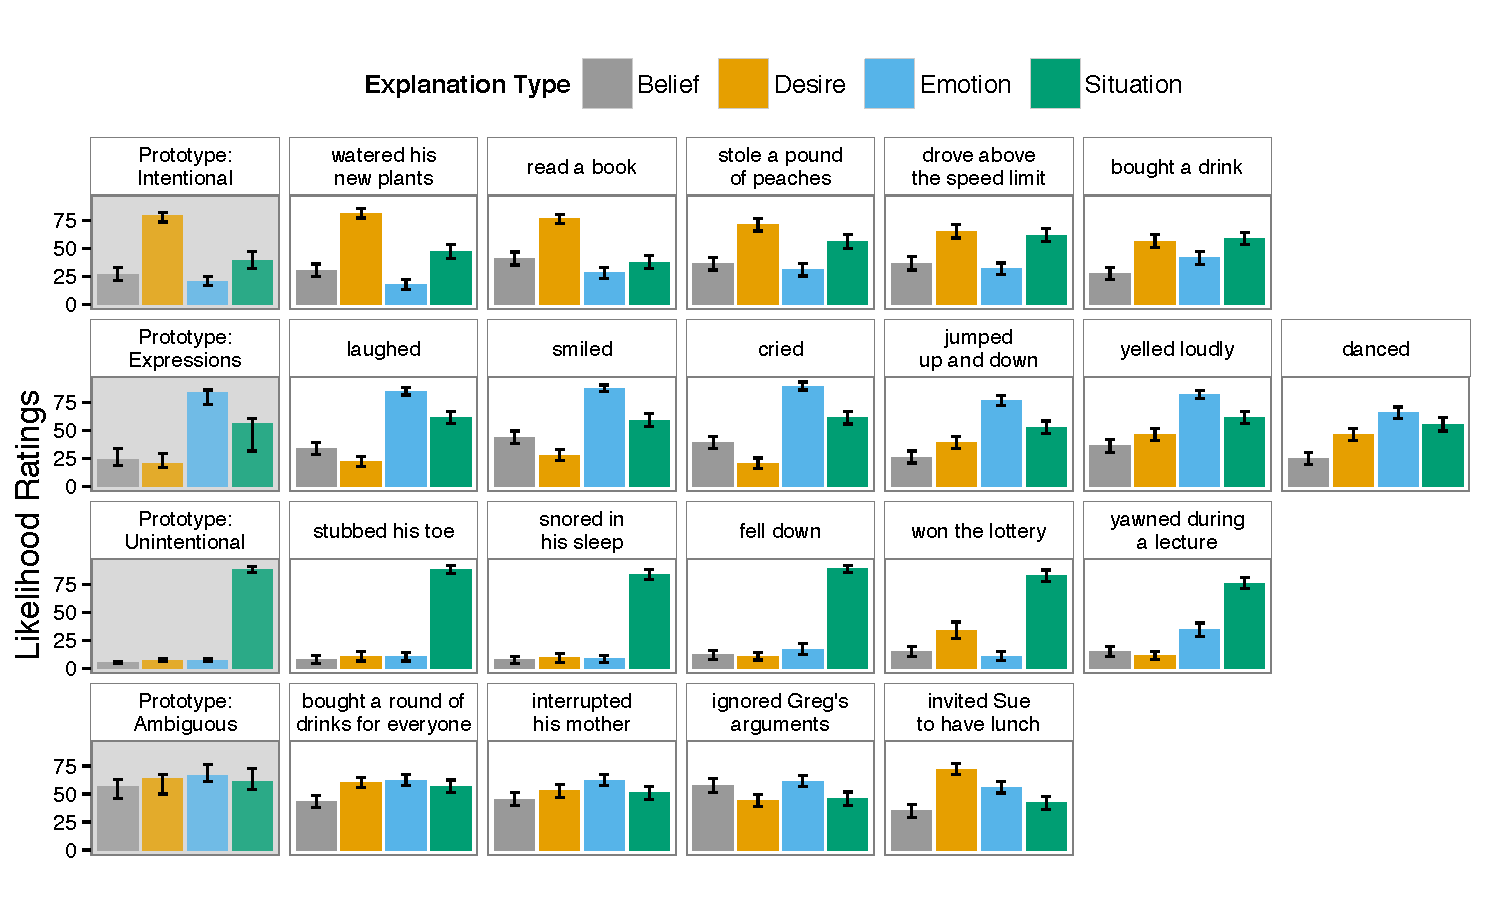
\includegraphics[width=1\linewidth]{images/study2Results.pdf}\end{center}
\caption{ Results of Study 2. Mean ratings of how likely each explanation type was to have caused the action. The left most column, shaded in grey, illustrate our a priori predictions. Error bars on empirical data indicate 95\% confidence intervals. }
\label{Study2ResultsFig}
\end{figure*}


\subsubsection{Stimuli Selection.} We selected a set of 20 actions, comprising a mix of 6 intentional actions, 6 emotional expressions, 5 unintentional behaviors, and 3 ambiguous behaviors. Of the 6 intentional actions, we chose 3 of them (``stole a pound of peaches"; ``invited Sue to have lunch"; and ``watered his new plants") from \citeA{Malle1999}'s study as they were previously rated as very highly intentional. We chose the 6 emotional expressions from the modal responses of Study 1a (i.e., from Table \ref{Study1aResultsTable}). We chose two unintentional behaviors (``yawned during a lecture", ``won the lottery") from \citeA{Malle1999}'s list, as they were rated as being low on intentionality. Finally, we chose 3 ``ambiguous" behaviors (``interrupted his mother"; ``ignored Greg's arguments"; ``drove above the speed limit"), all from \citeA{Malle1999}'s study, which were rated by some of their participants as being intentional, and others as being unintentional.
We predicted that the ambiguous behaviors would elicit medium endorsements across all explanation types.

\subsubsection{Participants and Procedures.} 
We recruited 100 participants through AMT (98\% had English as their native language; 1\% did not report).
First, participants were instructed about different types of explanations, with examples of each. (1) People have \textbf{thoughts} or beliefs about the way the world is that make them behave so (``Bob moved to Iowa because he \textbf{thinks} people are nice there"); 
(2) People feel certain \textbf{Emotions} that make them behave so, (``Bob ran away because he was \textbf{feeling} scared"); 
(3) People behave that way to achieve certain \textbf{Aims} (``Bob kicked the ball because he \textbf{wanted to} win the game"); and 
(4) People behave that way because of the \textbf{Situation} (``Bob shivered because it was cold outside").
%\ndg{make sure these are exactly as in expt. (some are grammatically odd -- due to shortening or what people actually saw?)}

Next, participants saw statements of the form ``Bob [\textbf{action}] because ...", followed by descriptions of four explanation types: (``... he was motivated by some thoughts or beliefs about the way the world is"; ``... he felt some emotions"; ``... he wanted to achieve some aims of his"; ``of some situational causes"). They then used continuous, 100 point sliders to rate how likely it was that the behavior was caused by each type of cause, from ``Not at all likely" to ``Extremely likely". Participants completed the 20 actions in a random order.


\subsubsection{Results.} 
Participants' mean ratings for each action, along with our a priori predictions, are shown in Figure. \ref{Study2ResultsFig}. 
By and large, participants' mean ratings across all the actions matched our predictions.

\red{What stats should I do?}
\ndg{yeah.. need to figure out some tests of the key claims in intro to this section: emotions can be decent causes of intentional actions, and desires can cause emotion expressions. also note some interesting posthoc findings, eg desires are better explanations of intentional actions than beliefs.}

\ndg{note that there's a sense in which these results support an intuitive theory with different kinds of actions: there are definitely different clusters of explanation profile here. this may be a confound of the design though, which chose different types on purpose. future work will have to take an unbiased sample of actions (somehow) and see whether there are still distinct explanation profiles.}


\ndg{if there is space i'd still love to see 2b which is elicitation and rating of specific explanations of each type. if we run out of space or time i guess this can be saved for a longer version....}



\section{Discussion}

Laypeople have rich intuitive theories of emotion that they use to explain many types of behavior, although emotion has often been neglected in work on intuitive theories. In this work, we explored some first steps into incorporating emotions into lay belief-desire psychology. Using both an unstructured free-response, sentence completion task (Study 1a/1b) and a more structured explanation rating task (Study 2), we show that people readily endorse emotions as causes of intentional actions, and moreover, judge beliefs and desires to be explanations of emotional expressions. Our results suggest the need to expand belief-desire psychology to appropriately capture how people make sense of emotion-driven and emotion-influenced actions.

Measuring lay theories is difficult, as one must elicit the lay participant's judgments without imposing too much of the researcher's own bias. We tried to mitigate this by using two varied approaches, but we must acknowledge the existing limitations. The space of emotions and the space of actions (intentional, emotional expressions, and unintentional) are both massive, and by focusing on a small set of emotions and actions, we risk the chance of conclusions being driven by idiosyncratic emotion or action choices. We note too that some of the modal actions that we observed in Study 1a (e.g., ``punched the wall") may be driven by cultural stereotypes. Future work should examine different ways of eliciting unbiased samples of actions and explanations.

There is obviously much more work to be done to fully elaborate on how emotions affect intentional actions in the lay theory. Borrowing ideas from empirical evidence on emotions, emotions might impact an agent's beliefs, by affecting their subjective judgments of probability \cite{Wright1992} or influencing the processing of novel information \cite{Forgas1995}. Alternatively, emotions might influence desires, by introducing new goals via approach/avoid motivations \cite{Carver2004}, or by introducing emotional states as regulatory goals in and of themselves \cite{Gross2006}. Finally, emotions might have a direct impact on intentional action that is independent of beliefs and desires; this possibility might be needed for lay explanations of ``rash" decisions (such as crimes of passion, like Othello). Future work should address all of these possibilities.

%How do emotions affect intentional action?
%Influence beliefs
%Influence desires
%Influence other than via beliefs/desires.
%All these are ripe for future work!


In summary, here, we have focused on lay explanations of behavior. This work builds towards a larger program of research on how humans use rich intuitive theories of emotion to reason about others---what we call Affective Cognition \cite{Ong2015AffCog}. Intuitive theories of emotion have broad and wide-reaching impact on all forms of social cognition, from understanding the family, friends and colleagues around us, to making attributions in moral and legal judgments. And of course, they help us enjoy a little theatre. 

%Using sentence completions to study intuitive theories



\section{Acknowledgments}

This work was supported in part by an A*STAR National Science Scholarship to DCO and by \red{[TODO:] XXX to NDG}.


\bibliographystyle{apacite}

\setlength{\bibleftmargin}{.125in}
\setlength{\bibindent}{-\bibleftmargin}

\bibliography{shakespeare_cogsci}




%In Study 1a/b, we examined participants' judgments of actions from several emotions, and we did not impose any formal structure on the type of actions that people generated (e.g., whether they were intentional actions or emotional expressions). In Study 2, we sought to test Figure \ref{ModelsOfBehaviorFig}c in a more hypothesis driven manner. First, we chose a set of actions (that span Intentional Actions, Emotional Expressions, and Unintentional Behavior), and specifically elicited Belief, Desire, Emotion, and Situational Factor explanations for these actions. We then collected, on a separate sample, ratings on the modal responses to each of these explanations. Under Figure \ref{ModelsOfBehaviorFig}c, we might hypothesize that (1) Beliefs and Desires will be rated highest as causes for Intentional Actions, although Emotion ratings will also be high, (2) Emotion ratings will be highest for Emotional Expressions, and ratings of Beliefs and Desires will also be high, and (3) For Unintentional Behavior, we should see high ratings for Situational Factor causes, and low ratings on other types of causes.
%
%\subsection{Generating lay explanations.} 
%To generate plausible lay explanations of behavior, we recruited 100 participants through AMT (97\% had English as their native language; 1\% did not report). Participants read about four different types of explanations for behavior: \textbf{thoughts} (i.e., beliefs about the state of the world), \textbf{emotions}, \textbf{aims} (i.e., desires), and \textbf{situational causes}. They read simple lay definitions of these four types of causes, and read examples of each (e.g. ``Bob moved to Iowa because he thinks people are nice there"). Then, participants saw statements and gave four different explanations for each statement, e.g. ``Bob [\textbf{action}] because he thought \underline{\hspace{3em}} (please give a thought)". Thus, whereas in Study 1b, we elicited only one explanation per action, here in Study 2a we prompted participants for 4 possible explanations per actions. We chose a set of 10 actions that consisted of a mix of 4 intentional actions (taken from \citeNP{Malle1999}), 3 unintentional actions (e.g. ``snored in his sleep"), and 3 emotional displays (from Study 1a: ``smiled", ``cried", and ``yelled"). The modal responses served as stimuli for the rating task, below.

% intentional actions after Malle 1999
%watered his new plants
%invited Sue to have lunch
%stole a pound of peaches
% drove above the speed limit

% smiled
% cried
% yelled

% slipped and fell
% snored in his sleep
% stubbed his toe

%\subsection{Rating Task}
%For the rating task, we recruited a separate group of 100 participants through AMT (X\% had English as their native language).


\end{document}
